% Submission: 4th eBPF Workshop (eBPF'26), co-located with ACM SOSP 2026
% Submission deadline: 2026-06-19
% Format: Research paper, 6 pages body + unlimited references
% Anonymity: double-blind for review submission

% \documentclass[sigconf,review,anonymous]{acmart}
\documentclass[sigplan,10pt,review,anonymous]{acmart}
\settopmatter{printfolios=true}
\pagestyle{plain}

% --- ACM metadata (anonymized for review; restore in camera-ready) ---
\setcopyright{none}
\acmConference[eBPF'26]{4th ACM SIGCOMM Workshop on eBPF and Kernel Extensions}{September 29, 2026}{Prague, Czech Republic}
\acmYear{2026}
\settopmatter{printacmref=false, printccs=false, printfolios=true}

\citestyle{acmnumeric}

% --- Packages ---
\usepackage{booktabs}
\usepackage{listings}
\usepackage{xcolor}
\usepackage{pifont}
\usepackage{xspace}
\usepackage{graphicx}
\usepackage[noend]{algpseudocode}
\usepackage{algorithm}

% --- Scoreboard marks for Table 4 (expressiveness) ---
% Use \partsym (not \partial) — \partial is the LaTeX kernel math symbol.
\newcommand{\yes}{\textcolor{green!55!black}{\ding{51}}}        % supported
\newcommand{\no}{\textcolor{red!70!black}{\ding{55}}}            % unsupported
\newcommand{\partsym}{\textcolor{orange!85!black}{$\sim$}}       % partial / awkward
\newcommand{\na}{\textcolor{gray}{\textemdash}}                  % not applicable

% --- Listings style for kunai DSL snippets ---
\lstdefinestyle{kunai}{
    basicstyle=\small\ttfamily,
    columns=fullflexible,
    breaklines=true,
    keepspaces=true,
}
% Tighten the vertical space above/below code listings.
\lstset{aboveskip=5pt, belowskip=3pt}

% --- Macros ---
\newcommand{\kunai}{Kunai\xspace}
\newcommand{\xdpninja}{xdp-ninja\xspace}
\newcommand{\TODO}[1]{\textcolor{red}{[TODO: #1]}}
\newcommand{\figref}[1]{Figure~\ref{#1}}

% Let column slack collect at the bottom instead of being stretched into
% the gaps around floats (acmart defaults to \flushbottom).
\raggedbottom

% Allow a little emergency stretch so long texttt identifiers do not
% poke past the column edge in the narrow two-column measure.
\setlength{\emergencystretch}{2em}

% Tighten the vertical space around floats and captions; acmart's
% defaults leave wide gaps between tables/figures and the body text.
\setlength{\textfloatsep}{10pt plus 2pt minus 2pt}
\setlength{\floatsep}{8pt plus 2pt minus 2pt}
\setlength{\intextsep}{10pt plus 2pt minus 2pt}
\setlength{\dbltextfloatsep}{10pt plus 2pt minus 2pt}
\setlength{\dblfloatsep}{8pt plus 2pt minus 2pt}
\setlength{\abovecaptionskip}{4pt}
\setlength{\belowcaptionskip}{2pt}

% Let a page hold more float area before deferring a float to a later
% page (the deferral is what leaves large gaps).
\renewcommand{\topfraction}{0.9}
\renewcommand{\bottomfraction}{0.8}
\renewcommand{\textfraction}{0.07}
\renewcommand{\floatpagefraction}{0.7}

\begin{document}

\title{Kunai: Toward a Verifier-Safe Layered DSL for Nested Encapsulation Packet Filtering on eBPF}

% --- Authors ---
% NOTE: the `anonymous' class option above suppresses all of the following
% and prints "Anonymous Author(s)" during review. These four blocks take
% effect only in the camera-ready (non-anonymous) build. Fill in real
% names/affiliations/emails before the final version.
\author{Takeru Hayasaka}
\affiliation{%
  \institution{Japan Advanced Institute of Science and Technology}
  \country{Japan}}
\additionalaffiliation{%
  \institution{BBSakura Networks Inc.}
  \country{Japan}}
\additionalaffiliation{%
  \institution{SAKURA internet Inc.}
  \country{Japan}}
\email{takeru.hayasaka@jaist.ac.jp}

\author{Satoshi Uda}
\affiliation{%
  \institution{Japan Advanced Institute of Science and Technology}
  \country{Japan}}
\email{zin@jaist.ac.jp}

\author{Ayako Hayasaka}
\affiliation{%
  \institution{Independent Researcher}}
\email{ternbusty.dev@gmail.com}

\author{Fourth Author}
\affiliation{%
  \institution{Kyoto University}
  \country{Japan}}
\email{kotani@media.kyoto-u.ac.jp}

\begin{abstract}
Packet capture and network debugging require selecting the packets
of interest early, inside the Linux kernel. However, pcap-filter,
tcpdump's filter language, has no syntax for nested
encapsulation, repeated occurrences of the same protocol, or the
variable-length lists and options whose field offsets change from
packet to packet. Running a filter in the kernel additionally
requires emitting bytecode that the Linux eBPF verifier accepts. For
such expressive filters this is difficult, since a naive lowering is
rejected. We present \kunai, a packet-filter DSL together with a compiler that
lowers its expressions to eBPF bytecode. A \kunai expression
describes a packet's layer structure and field conditions together,
and resolves each field's offset and type from
protocol definitions written in a subset of P4. The compiler records
every header's start offset at run time, bounds each variable-length
scan by a compile-time constant, and places a verifier-compliant
bounds check before every packet read. We evaluated \kunai on filters spanning GTP-U, SRv6, Geneve, and TCP
options. The generated bytecode was accepted by the verifier across
six kernels (Linux 6.1--7.0) on both the XDP and tc attach points, matched
and rejected the intended packets, and, where pcap-filter can express
the filter, ran within a few percent of pcap-filter in per-packet
processing cost. These
results show that \kunai enables the
Linux kernel to execute protocol-aware filters beyond what
pcap-filter's structured syntax can express.
\end{abstract}

\keywords{eBPF, XDP, packet filtering, domain-specific language, P4,
  kernel verifier, packet capture, network debugging}

\maketitle

\section{Introduction}
\label{sec:intro}

Packet capture is a fundamental tool for debugging, troubleshooting,
and fault analysis of network systems. As link bandwidth and traffic
volume continue to increase, a software capture that forwards every
packet to user space for storage no longer scales~\cite{braun2010capture}. A capture tool must therefore select only
the packets relevant to its purpose as early as possible, ideally
inside the kernel datapath~\cite{papadogiannakis2013scap}. The de-facto language for this purpose has
long been tcpdump/libpcap’s
pcap-filter~\cite{pcapfilter_man,mccanne1993bpf}.

Packet structures whose field locations cannot be determined
statically are common in modern networks. Examples include the inner
headers of GRE, GTP-U, and Geneve tunnels, repeated occurrences of the
same protocol, and variable-length structures such as SRv6 segment
lists and TCP options~\cite{rfc2784,gtp_3gpp,rfc8754,rfc8926,rfc9293}. In these
cases, the location of the target field depends on packet contents and
changes from packet to packet.

Existing packet-filter languages provide limited support for such
structures. pcap-filter expresses conditions over fixed L2–L4 header
fields, but it cannot naturally express nested encapsulation,
repeated protocol occurrences, or variable-length protocol structures.
More expressive languages such as the Wireshark display
filter~\cite{wireshark_dfref} can express conditions over nested
encapsulation and variable-length structures. However, they operate on
parsed packets in user-space memory and cannot execute directly in the
kernel datapath. Existing tools thus leave a gap, and user studies of
packet-analysis tools identify protocol coverage and filter
expressiveness as open problems~\cite{sultana2024survey}.

To execute a filter inside
the Linux kernel, it must also be compiled into eBPF bytecode that the
verifier accepts~\cite{kernel_verifier,ebpf_loops,gershuni2019prevail}.
The verifier requires every packet access to be proven safe. For
fields located behind nested encapsulation or variable-length
structures, the required offset is often known only at run time. As a
result, a naive lowering produces packet accesses whose range the
verifier cannot prove, causing the generated bytecode to be rejected.

Even verifier-aware P4-to-eBPF compilers such as
p4c-xdp~\cite{tu2018p4cxdp} target fixed protocol pipelines rather than
filter expressions over arbitrary encapsulation. Existing systems thus
provide either expressive packet descriptions or verifier-accepted
execution, but not both.

We present \kunai, a verifier-safe packet-filter DSL and compiler for
nested encapsulation and variable-length protocol structures. \kunai
describes packet structure and filter conditions through a
protocol-aware \emph{layer-chain} representation and resolves field
references using protocol definitions written in a subset of
P4~\cite{p4spec}.

The compiler lowers dynamic packet accesses into forms that the
verifier can prove safe. It records the start offset of each parsed
header during packet traversal and lowers every variable-length walk
into a compile-time bounded form. These code-generation patterns
translate field references beyond nested encapsulation and
variable-length structures into verifier-accepted eBPF bytecode. We
use the term \emph{verifier-safe} in the sense of Solleza et
al.~\cite{solleza2025verifiersafe}: a well-formed filter should
compile to bytecode that the verifier accepts.

We evaluated \kunai on filters spanning GTP-U, SRv6, Geneve, and TCP
options. The generated bytecode was accepted by the verifier across
six Linux kernel versions (6.1–7.0) on both the XDP and tc attach points,
matched and rejected packets as intended, and incurred only modest
overhead relative to pcap-filter where equivalent filters could be
expressed. These results showed that such packet filters compiled into
verifier-accepted eBPF programs that matched and rejected packets as
intended.
\section{Related Work}
\label{sec:related}

Existing packet filters trade expressiveness for in-kernel execution.
tcpdump/libpcap's pcap-filter descends from the Packet
Filter~\cite{mogul1987packetfilter} and the BSD Packet
Filter~\cite{mccanne1993bpf} and runs L2--L4 conditions in the kernel.
As \S\ref{sec:intro} noted, it has no syntax for repeated protocols or
for walking variable-length lists such as an SRv6 segment list or TCP
options by field name; the more expressive Wireshark display
filter~\cite{wireshark_dfref} runs only in userspace. Tools that capture
at the XDP layer do not close this gap. xdpcap runs filters in the
kernel, but its filter language is still
pcap-filter~\cite{cloudflare2019xdpcap}, inheriting the same limit;
xdpdump has no in-kernel filter, capturing via fentry/fexit and
leaving matching to tcpdump~\cite{xdptools_xdpdump}. Neither selects
packets in the kernel by a field condition past nested encapsulation.

Prior work on encapsulation-aware filters includes NetPDL/NetPFL and
pFSA/xpFSA. NetPDL/NetPFL connect a description of protocol headers
with tunnel-aware filter
expressions~\cite{risso2006netpdl, ciminiera2010netpfl}. pFSA/xpFSA
represent the order in which headers appear within an encapsulation
as state transitions and formalize the composition of filters and
field access~\cite{leogrande2015pfsa, cerrato2018xpfsa}. These share
our goal of bringing nested encapsulation into the filter expression,
but do not emit eBPF bytecode for the Linux kernel data path. They
therefore lack the in-kernel execution this paper requires.

Among combinations of P4 and eBPF, p4c-ebpf and p4c-xdp compile a P4
data-plane program to Linux eBPF / XDP /
tc~\cite{p4c_ebpf, tu2018p4cxdp}, and Simon et
al.~\cite{simon2024honey} embed dynamically loaded eBPF inside a P4
pipeline.
These move an entire P4 pipeline to the target rather than returning
per-packet match/reject from a filter expression; \kunai instead uses P4
only as a protocol definition, not as a data-plane language~\cite{p4spec}.

We adopt the recent \emph{verifier-safe} goal argued by Solleza et
al.~\cite{solleza2025verifiersafe}: a kernel-extension DSL should
compile every well-formed program to bytecode the verifier accepts.
\kunai is a concrete instance of that position for packet filtering over
nested encapsulation: rather
than restricting an existing DSL, we identify the code-generation
patterns the goal demands when a filter reaches past variable-length
structure (\S\ref{sec:codegen}).

The work above has separately addressed packet-filter execution, filter
expression over nested encapsulation, P4-to-eBPF compilation, and the
goal of verifier-safe lowering. \kunai joins two of these: it brings
nested encapsulation and variable-length structure into the filter
expression and compiles the result into bytecode the verifier accepts,
generalized across the protocols declared in the P4 subset
(\S\ref{sec:codegen}).

\section{Design}
\label{sec:design}

\subsection{Overview}
\label{sec:overview}

\kunai combines expressive packet filtering with verifier-safe
execution through three components: a protocol-aware filter language,
protocol definitions written in a subset of P4, and verifier-safe code
generation. The filter language describes packet structure and field
conditions, the protocol definitions describe protocol layouts, parser
transitions, and variable-length structures, and the code-generation
stage combines both to produce verifier-accepted eBPF bytecode.
\figref{fig:arch} shows the overall structure.

The compiler takes two inputs, a \kunai filter expression and a set of
protocol definitions written in a subset of P4. It first validates the
layer-chain, resolves field references against the protocol
definitions, and records the information required for later code
generation, rejecting references to non-existent fields, ambiguous
references to repeated protocols, and comparisons whose types do not
match.

The compiler then generates eBPF bytecode that evaluates the filter
condition and returns a match/reject result. A host BPF program
placed at an attach point such as XDP~\cite{hoiland2018xdp},
tc~\cite{tc_man}, or fentry/fexit embeds this bytecode. Under this
split of responsibilities, \kunai handles filter analysis and
bytecode generation, while the host program handles
attach-point-specific context access and follow-on actions such as
capture or drop.

\begin{figure}[t]
  \centering
  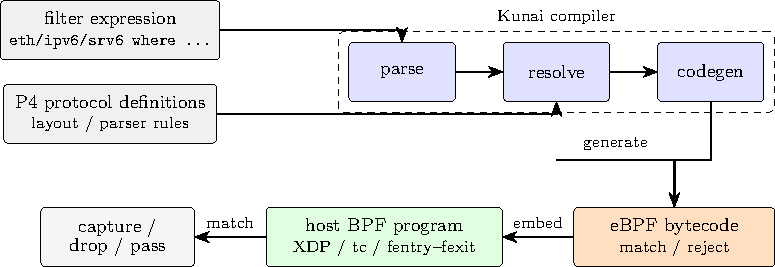
\includegraphics[width=0.8\columnwidth]{figures/fig_arch.pdf}
  \caption{Overview of \kunai.}
  \label{fig:arch}
\end{figure}

\subsection{What the DSL Expresses}
\label{sec:dsl}

The \kunai DSL describes a packet's layer structure and field
conditions as a single filter expression; \figref{fig:grammar} shows
an excerpt of the grammar; the full grammar is available in the
project repository.\footnote{\url{https://github.com/(redacted for review)}}

\begin{figure}[t]
\begin{lstlisting}[basicstyle=\scriptsize\ttfamily,breaklines=true,columns=fullflexible]
filter       ::= layer-chain where-clause?
layer-chain  ::= layer ('/' layer)*
layer        ::= layer-atom quantifier?
layer-atom   ::= proto-name ('@' label)? predicate?
               | '(' layer ('|' layer)+ ')'
quantifier   ::= '?' | '+' | '*' | '{' INT '}' | '{' INT ',' INT '}'
predicate    ::= '[' comparison (',' comparison)* ']'
where-clause ::= 'where' bool-expr
bool-expr    ::= comparison | quant-atom
               | '(' bool-expr ')' | bool-expr bool-op bool-expr
comparison   ::= field-ref op value
quant-atom   ::= ('any' | 'all') '(' bool-expr ')'
field-ref    ::= ident index? ('.' ident index?)*
\end{lstlisting}
\caption{Excerpt of the \kunai filter-expression grammar.}
\label{fig:grammar}
\end{figure}

A layer-chain lists, with \texttt{/}, the order in which protocols
appear in the packet, and can also express optional layers,
repetition, and choice. The \texttt{where} clause is a condition over
the fields of layers in the chain and of auxiliary headers and lists.
\kunai resolves a field reference into one of the forms in
Table~\ref{tab:fieldref}; there, \texttt{<stack>} is not a literal but
the name of an auxiliary header list given in the protocol definition,
such as \texttt{segments} or \texttt{exts}.

\begin{table}[htbp]
  \centering\footnotesize
  \setlength{\tabcolsep}{4pt}
  \begin{tabular}{@{}ll@{}}
    \toprule
    Reference form (example) & Meaning \\
    \midrule
    \texttt{proto.field} (\texttt{tcp.dport}) & primary field of a protocol unique in the chain \\
    \texttt{label.field} (\texttt{inner.dst}) & field of a layer carrying a label (\texttt{@inner}) \\
    \texttt{proto.aux.field} & field of an optional or auxiliary header \\
    \texttt{proto.<stack>[N].field} & static index into an auxiliary header list \\
    \texttt{proto.<stack>.field} & element being walked in \texttt{any()}/\texttt{all()} \\
    \texttt{proto.options.NAME.field} & TCP / IPv4 option lookup \\
    \bottomrule
  \end{tabular}
  \caption{Field-reference forms \kunai resolves.}
  \label{tab:fieldref}
\end{table}

\kunai interprets a field reference inside a bracket predicate as
relative to that layer. In the \texttt{where} clause, references name
the layer explicitly, as in \texttt{proto.field} or
\texttt{label.field}.

When the same protocol appears more than once in a chain,
\texttt{proto.field} alone does not determine which layer to read.
For example, when a chain contains both an outer and an inner IPv4 header,
\texttt{ipv4.dst} does not uniquely identify which destination field
is meant. \kunai rejects such a reference before code generation and
requires a label-qualified reference. A filter on the inner IPv4
destination of a GTP-U tunnel, for example, is written as follows.

\begin{lstlisting}[style=kunai]
eth/ipv4@outer/udp/gtp/ipv4@inner/tcp where inner.dst == 10.0.0.1
\end{lstlisting}

The chain before \texttt{where} lists the layers to traverse, from
Ethernet through an outer IPv4 header, UDP, GTP, an inner IPv4 header,
to TCP, and the \texttt{where} clause gives the field condition checked
once the chain matches, here that the inner IPv4 header's destination
equals \texttt{10.0.0.1}. Here \texttt{@outer} and \texttt{@inner} distinguish the two IPv4
layers. Because \texttt{inner.dst} uniquely names the destination
field of the inner IPv4 header, \kunai can determine which field to read even
though the same \texttt{ipv4} header appears twice.

Variable-length lists are handled with \texttt{any()} and
\texttt{all()}. A filter that matches a packet whose SRv6 segment list
contains a given address, for example, is written as follows.

\begin{lstlisting}[style=kunai]
eth/ipv6/srv6 where any(srv6.segments.addr == fc00::1)
\end{lstlisting}

The scan target of \texttt{any()} and \texttt{all()} is the auxiliary
header list referenced without an index inside the expression, and
there must be exactly one such target list. The same list may be
referenced several times; for example,
\texttt{any(srv6.segments.addr == fc00::1 or srv6.segments.addr ==
fc00::2)} is valid. An \texttt{any()} or \texttt{all()} that references no un-indexed list, or
two different ones, is rejected at the analysis stage rather than
walking one of them. A quantifier that appears to walk two
lists therefore cannot be written. \kunai evaluates the inner condition
against each element of the list. The walk requires a field giving the
element count, the width of each element, a way to advance to the next
element, and a stop condition; the protocol definition supplies these.
TCP options and GTP extension headers are handled the same way when
the protocol definition carries this information.

Through these constructs, the \kunai DSL specifies, within one filter
expression, the order in which headers appear, the disambiguation of
repeated protocols, and the target of a variable-length walk. Code generation
uses this information to translate each field access into an offset
from the layer's start and a bit width.

\subsection{Protocol Definitions via a P4 Subset}
\label{sec:p4subset}

\kunai describes protocol headers and parser rules in a subset of
P4~\cite{p4spec,doenges2021petr4,bosshart2014p4}. Existing P4
descriptions then serve as a reference, and \kunai avoids building the
syntax checker, parser, and tooling that a bespoke protocol-description
language~\cite{mccann2000packettypes,pang2006binpac} would require.

The P4 subset \kunai handles is limited to the parts that describe
header layout and parser transitions. \figref{fig:p4srv6} gives the
SRv6 definition, used by the \texttt{any()} example in \S\ref{sec:dsl}
and filter F8 in \S\ref{sec:eval}.

\begin{figure}[t]
\begin{lstlisting}[basicstyle=\scriptsize\ttfamily,breaklines=true,columns=fullflexible]
// headers, extern ParserCounter, const SRV6_ROUTING_TYPE elided
const bit<8> KUNAI_SRV6_IPV6_NEXT_HEADER = 43;   // IPv6 -> SRv6
parser SRv6Parser(packet_in pkt, out srv6_h hdr,
                  out srv6_seg_h[8] segments) {
  ParserCounter() pc;
  state start {
    pkt.extract(hdr);
    pc.set((bit<8>)(hdr.last_entry + 1));   // segment count
    transition select(hdr.routing_type) {
      SRV6_ROUTING_TYPE: walk;  default: reject; } }
  state walk {
    transition select(pc.is_zero()) { true: accept; false: consume_seg; } }
  state consume_seg {
    pkt.extract(segments.next);   // push one 16-byte segment
    pc.decrement(1);  transition walk; } }
\end{lstlisting}
\caption{SRv6 protocol definition in the \kunai P4 subset.}
\label{fig:p4srv6}
\end{figure}

A definition gives \texttt{header} layouts, a \texttt{transition
select} dispatch such as IPv6 to SRv6 on \texttt{routing\_type}, and a
parser walk over a variable-length list. For SRv6 the
\texttt{ParserCounter} is seeded with \texttt{last\_entry + 1} and one
16-byte segment is extracted per iteration, so the element count and
the \texttt{segments} base follow from the walk itself with no \kunai
annotation, and the array capacity bounds the iteration count for the
verifier. In this way, a protocol definition describes layout,
dispatch, and walk metadata within P4 syntax, and adding one extends
the set of supported protocols without changing the compiler itself.

\section{Verifier-Constrained Code Generation}
\label{sec:codegen}

This section describes how \kunai lowers a filter expression into the
packet accesses, loops, and bounds checks that the Linux eBPF verifier
accepts. When nested encapsulation or a variable-length structure makes a
subsequent header's start offset vary per packet, reading a field at
that run-time offset leaves its range unprovable to the verifier. As a
result, the bytecode is rejected. The code generation below avoids it.

The difficulty is not detecting that an offset is dynamic but
lowering the read, the same way for every layer past a variable-length
one and for every protocol in the P4 subset, into a form the verifier
accepts. \kunai's code generation does this by recording each changing
header's start offset at run time (\S\ref{sec:offset}) and walking
variable-length structures such as SRv6 segments and TCP options under a
compile-time bound (\S\ref{sec:bounded}), with a verifier-compliant
bounds check before every packet read.

\subsection{Recording Header Start Offsets Explicitly}
\label{sec:offset}

\kunai records each header's start offset at run time and reads a
field as a relative offset from that start. Consider again the GTP-U
inner-IPv4 filter of \S\ref{sec:dsl}: \texttt{inner.dst} is not at a
fixed offset, since the start of the inner IPv4 changes with the outer
IPv4 length, the GTP optional fields, and the structure of the
encapsulation.

A fixed compile-time offset does not suffice: if the variable-length parts
before the field (GTP optional fields or IPv4 options) are non-empty,
it reads the wrong bytes. The offset must be computed at run time. But a
run-time offset against the native-XDP packet pointer
(\texttt{PTR\_TO\_PACKET}) is one the verifier cannot bound. The
verifier therefore cannot prove the read stays within \texttt{data\_end}
and rejects the bytecode.

\kunai detects this boundary at the resolve stage and marks every
layer after one with a variable-length layout as a run-time offset.
The generated eBPF bytecode then records each header's start offset
into a stack slot as it traverses the header at run time.
\figref{fig:layerstart} illustrates this offset recording and a
bounds-checked load that uses the recorded offset.

\begin{figure}[htbp]
  \centering
  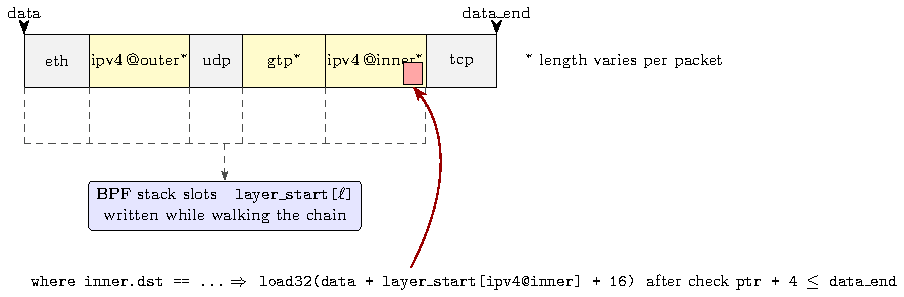
\includegraphics[width=\columnwidth]{figures/fig_layerstart.pdf}
  \caption{Recording each header's start offset into a stack slot, and
  reading \texttt{inner.dst} as a bounds-checked load at layer-start
  $+$ field offset.}
  \label{fig:layerstart}
\end{figure}

Every field access takes the same form: \kunai loads the layer's start
offset, adds the field offset and width, checks the access against
\texttt{data\_end}, loads, and compares. Because type-mismatched
comparisons and a \texttt{proto.field} reference under a repeated
protocol are already rejected at the analysis stage of
\S\ref{sec:overview}, code generation need only emit this bounds-checked
load, even for a chain whose subsequent-header start changes at run time.

\subsection{Lowering Variable-Length Structures to Bounded Bytecode}
\label{sec:bounded}

Because the element count or the length of each element changes per
packet, variable-length structures such as SRv6 segments and TCP
options cannot be walked at a fixed offset. \kunai puts the walk into a
verifier-accepted form by translating it into bytecode with a
compile-time constant bound.

\kunai generates the walk as one of two kinds of bytecode, chosen by
the bound and applied uniformly to chain quantifiers and
\texttt{any()}/\texttt{all()} aux-list walks. A small compile-time bound
within a fixed threshold is unrolled in place. A larger or unbounded one
is lowered to a
\texttt{bpf\_loop} callback with a constant
bound~\cite{bpf_loop_helper}, whose size no longer grows with the
bound; this case covers a parser-machine self-loop, an unbounded chain
quantifier, and a chain or aux-list walk past the threshold.
An SRv6 segment walk and a large MPLS stack take the same lowering.

Algorithm~\ref{alg:walk} gives the shared skeleton; the two lowerings
below instantiate its \textsc{stop}, \textsc{stride}, and \textsc{step}
steps, each emitted by its own generator.

\begin{algorithm}[htbp]
  \caption{Bounded walk skeleton; \textsc{stop}, \textsc{stride}, and
  \textsc{step} are instantiated per structure.}
  \label{alg:walk}
  \begin{algorithmic}[1]
    \Require $data,\ data\_end,\ base,\ cap$; \textsc{stop}, \textsc{stride}, \textsc{step} per structure
    \State $r \gets \bot$;\ $off \gets base$
    \For{$i \gets 0$ \textbf{to} $cap-1$} \Comment{$cap$: compile-time bound}
      \State \textbf{if} $\textsc{stop}(i, off)$ \textbf{then break} \Comment{count reached, or end/END/malformed}
      \State $ptr \gets data + off$
      \State \textbf{if} $ptr + w > data\_end$ \textbf{then break} \Comment{$w$: bytes read; bounds check}
      \State $r \gets \textsc{step}(ptr)$; \textbf{break if} $r$ decides \Comment{compare, or record option}
      \State $off \gets off + \textsc{stride}(ptr)$ \Comment{constant, or this option's length}
    \EndFor
    \State \Return $r$
  \end{algorithmic}
\end{algorithm}

\kunai instantiates this skeleton in two ways, chosen by the structure
rather than the protocol. A \emph{counted aux-list walk} handles a list
of fixed-size elements with a run-time count, such as the SRv6 segment
list: \textsc{stop} is $i \geq count$, \textsc{stride} is the constant
element width, and \textsc{step} compares the element field to the
target and decides the walk on a match. For the SRv6 segment filter of
\S\ref{sec:dsl}, \texttt{base = srh\_start + SRH\_FIXED\_SIZE},
\texttt{stride = width = 16}, \texttt{count = last\_entry + 1} (the SRv6
parser's segment-walk seed in \S\ref{sec:p4subset}), and
\texttt{target = fc00::1}.

A \emph{TLV self-loop} handles options that differ in kind and length,
such as TCP options, where a reference like
\texttt{tcp.\allowbreak options.\allowbreak MSS.\allowbreak value} sits
at no fixed offset. Here \textsc{stride} is each option's length,
read at the cursor; \textsc{stop} fires when the cursor reaches the end
of the options, on an END option, on a malformed option (\texttt{len < 2}
or \texttt{cursor + len > options\_end}), or at the iteration bound; and
\textsc{step} dispatches on the option kind and records the position of
the referenced option, which the \texttt{where} clause then reads after
the walk. An option field is loaded only after checking that its option
header stays within the packet window.

In either instantiation, and in either the fixed-unrolling or the
\texttt{bpf\_loop} form, the bound is a compile-time constant and a
bounds check precedes every packet load. The verifier can therefore
confirm both the loop bound and the range of every packet access.

So that the generated bytecode is accepted across kernel versions,
\kunai avoids instructions available only on newer versions. For
byte-order conversion, for example, it uses the \texttt{BPF\_END}
instruction, available on older versions, rather than the
\texttt{BSWAP} instruction introduced in 6.6~\cite{bpf_isa}.

These two patterns are not specific to \kunai but are what a
verifier-safe lowering of nested, variable-length filters requires.
\emph{Recorded-base addressing} reads each field as a recorded
layer-start base plus a static offset, spilling the base to a stack slot
during traversal, which makes an otherwise unprovable run-time read
provable. \emph{Constant-bounded scanning} bounds every variable-length
walk by a compile-time cap, unrolled when small and lowered to a
\texttt{bpf\_loop} callback when large; both the trip count and each
read are therefore provable. Only the base, run-time or compile-time constant,
varies between reads; the read shape is uniform, and \kunai selects the
lowering from the structure's shape, not its protocol name. GTP-U,
SRv6, Geneve, and TCP options therefore need no per-protocol code in
the generator.

\section{Evaluation}
\label{sec:eval}

We evaluated \kunai from three angles. First, whether the packet
structures \kunai targets can be written as filter expressions
(\S\ref{sec:eval-expr}). Second, whether the generated bytecode is
accepted by the eBPF verifier and matches/rejects as expected
(\S\ref{sec:eval-accept}). Third, the instruction count and run-time
cost of the generated bytecode (\S\ref{sec:eval-cost}).

\subsection{Method and Filter Set}
\label{sec:eval-method}

The evaluation uses ten filters, F1--F10, listed in Table~\ref{tab:filterset}. F1--F6 target basic protocol
headers such as Ethernet, VLAN, IPv4/IPv6, TCP, and ICMP, while
F7--F10 target nested headers and variable-length structures whose
start cannot be fixed at a constant offset. It lists each filter's
\kunai expression and the raw eBPF instruction count of the bytecode
\kunai generates, together with the count for the same filter compiled
from pcap-filter to eBPF through cBPF~\cite{mccanne1993bpf} using
cbpfc~\cite{cloudflare_cbpfc}, a cBPF-to-eBPF compiler. We refer to this latter count as the
pcap-filter baseline in the rest of the evaluation.

\begin{table*}[t]
  \centering\small
  \begin{tabular}{@{}llrr@{}}
    \toprule
    & & \multicolumn{2}{c}{raw insns} \\
    \cmidrule(l){3-4}
    ID & \kunai expression & \kunai & pcap-filter \\
    \midrule
    F1  & \texttt{eth/ipv4/tcp where tcp.dport == 443} & 199 & 42 \\
    F2  & \texttt{eth/ipv4[src==10.0.0.0/8]/tcp where tcp.dport == 80} & 209 & 36 \\
    F3  & \texttt{eth/ipv6[src==2001:db8::/32]/tcp} & 338 & 23 \\
    F4  & \texttt{eth/vlan[tci==100]/ipv4/tcp where tcp.dport == 80} & 215 & 51 \\
    F5  & \texttt{eth/qinq/vlan/ipv4/tcp where tcp.dport == 80} & 217 & \na \\
    F6  & \texttt{eth/ipv4/icmp where icmp.type == 8} & 85 & 31 \\
    F7  & \texttt{eth/ipv4@outer/udp/gtp/ipv4@inner/tcp where inner.dst == 10.0.0.1} & 405 & \na \\
    F8  & \texttt{eth/ipv6/srv6 where any(srv6.segments.addr == fc00::1)} & 332 & \na \\
    F9  & \texttt{eth/ipv4@outer/udp/geneve/eth/ipv4@inner/tcp where inner.dst == 10.0.0.1} & 351 & \na \\
    F10 & \texttt{eth/ipv4/tcp where tcp.options.MSS.value == 1460} & 231 & \na \\
    \bottomrule
  \end{tabular}
  \caption{Evaluation filter set and raw eBPF instruction counts.
  F7--F10 target nested headers and variable-length structures. The
  pcap-filter column is the eBPF compiled from each filter via cBPF;
  \na\ marks those pcap-filter cannot express.}
  \label{tab:filterset}
\end{table*}

To exercise the DSL syntax more broadly, we hand-constructed a separate
regression suite of 77 filter expressions, at least one per syntactic
feature of the DSL. The suite covers bracket
predicates, arithmetic in the \texttt{where} clause, quantified
layers, heterogeneous-size alternations, label disambiguation, and
aux-walks, spanning a wider syntactic range than F1--F10. Its verifier
acceptance and per-packet match/reject correctness are reported in
\S\ref{sec:eval-accept}.

To evaluate these filters, we embedded the generated bytecode in a
host BPF program and placed it at the XDP and tc attach points. The
remaining subsections use this filter set and regression suite
throughout.

\subsection{Expressiveness}
\label{sec:eval-expr}

We compared whether F1--F10 can be written in pcap-filter, the filter
language that runs in the kernel, and in \kunai. Because pcap-filter
has byte-offset access, the one expressiveness axis \kunai does
not follow (\S\ref{sec:limitations}), a hand-written
condition can sometimes be built for a specific packet layout. It does
not, however, provide as filter syntax the order of headers, an
arbitrary element of a variable-length list, repeated occurrences of
the same protocol, or a named reference to an inner header.

\textbf{Result:} F1--F6 were writable in both; only
F5 (QinQ) behaved in pcap-filter in a way that depended on the
capture environment, since NIC VLAN offload can strip the tag from the
bytes. The two diverge at F7--F10. The inner IPv4 header of F7 (GTP-U)
and F9 (Geneve) sits at no fixed offset, shifted per packet by GTP
optional fields and extension headers or by a Geneve inner Ethernet
header; F8 (SRv6) requires looping over an arbitrary segment-list
element; and F10 (TCP MSS) requires an option walk rather than a
byte-offset approximation. None of these is expressible as pcap-filter
syntax, whereas \kunai writes all of F1--F10 directly through the
labeled layer-chains, \texttt{any()}/\texttt{all()} quantifiers, and
option-field walks listed in Table~\ref{tab:filterset}.

\subsection{Verifier Acceptance and Correctness}
\label{sec:eval-accept}

We made two checks of the code generation of \S\ref{sec:codegen}:
first, that the generated bytecode is accepted by the eBPF verifier;
second, that the accepted bytecode matches and rejects as expected.

For acceptance, we loaded the bytecode generated from F1--F10 and the
regression suite onto six kernels (Linux 6.1, 6.6, 6.12, 6.15, 6.18,
7.0) at both the XDP and tc attach points. The instructions and
helpers the verifier accepts differ across kernel versions, but because
\kunai avoids version-dependent instructions as described in
\S\ref{sec:codegen}, the same bytecode was accepted unchanged on all
six versions.

At tc, the kernel extracts the outer VLAN tag into skb metadata before
the program runs. \kunai therefore rejects at compile time a filter that
reads a VLAN/QinQ field from packet bytes. An optional, predicate-free
tag stays matchable. Because at most one tag remains in the bytes,
\texttt{eth/vlan?/...} takes its skip path and matches untagged,
single-tagged, and QinQ frames without reading the stripped tag. This is
a compile-time restriction, not a verifier rejection. We excluded from
the tc loads only the field-reading forms, 2 of F1--F10 and 3 of the
regression suite, and performed 1014 loads across six kernels $\times$ 2
hosts, all accepted.

Next, we fed the generated bytecode actual packets (matching,
non-matching, and malformed) and checked the match/reject result. For
Geneve we varied \texttt{opt\_len} from 0 upward to confirm the inner
offset resolves past the skipped options, with truncated and malformed
frames throughout, and the bytecode returned the expected verdict in
every case. The regression suite was verified at two levels: all 77
expressions loaded on the verifier, and 74 of them were also checked for
match and reject correctness at the packet level; the 3 capture-clause
expressions were load-only, since their verdict equals the base chain. For the five filters both
languages express (F1 to F4 and F6) we also cross-checked \kunai against
libpcap, the engine behind tcpdump, on the same packets, and the
verdicts agreed throughout, an independent reference beyond the
hand-built expectations.

\textbf{Result:} These two checks show that the code generation of \S\ref{sec:codegen}
lowered the target filters into bytecode accepted across six kernels
$\times$ 2 hosts and traversed packet headers correctly.

\subsection{Instruction Count and Run-Time Cost}
\label{sec:eval-cost}

We first evaluate a filter's cost by the instruction count of the
generated eBPF bytecode, listed per filter in
Table~\ref{tab:filterset}. The instruction count is the static size of
the bytecode and is comparable regardless of the measurement
environment; a 64-bit immediate load is counted as two instructions
for both \kunai and pcap-filter. On the F1--F4 and F6 filters that
pcap-filter can also express, \kunai generated 2.7$\times$ to
14.7$\times$ as many instructions, the largest gap arising at the IPv6
prefix match of F3.

Because every variable-length walk is bounded at compile time, a
filter's instruction count grows with that bound, not with the packet: a
chain quantifier adds about 16 instructions per unit of cap while it
unrolls, then flattens once it lowers to a \texttt{bpf\_loop} callback,
and each stacked SRv6 segment walk, itself such a callback, adds a fixed
${\approx}68$. Even eight stacked walks stay near 800 instructions, three
orders of magnitude below the verifier's roughly one-million-instruction
limit.

To see whether this appears at run time, we connected a traffic
generator to a device under test (DUT) over 100\,GbE and attached a
native XDP program that evaluates the filter and returns
\texttt{XDP\_DROP} on every packet. The DUT runs Linux 6.15 with the
BPF JIT on an Intel Xeon 8362 and an E810 NIC. Unlike the acceptance
measurements, which cover six kernels at both the XDP and tc attach
points, the run-time figures below use this single Linux 6.15
configuration. As in an operational
fentry/tc observer, the program first copies the packet head into a
per-CPU scratch window; this copy alone lowered the rate by 6.7\%
even with no filter. We therefore measured each filter's cost as the
processing-rate reduction relative to that same-copy accept-all
baseline.

\figref{fig:datapath} shows the per-filter processing-rate reduction.
We measured at the 64-byte line rate and repeated each cell ten times;
every standard deviation was at most 0.4.

\textbf{Result:} The reduction for the basic
filters F1--F6 was 0--1.7\%, near 0\% for F6. The \kunai-only
filters F7--F10 were 3.9--7.4\%, with
F8, whose SRv6 segment list is walked by a \texttt{bpf\_loop} callback,
the largest at 7.4\%. For
F1, writable in both \kunai and pcap-filter, the difference between
the two was only 0.7\%.

\begin{figure}[htbp]
  \centering
  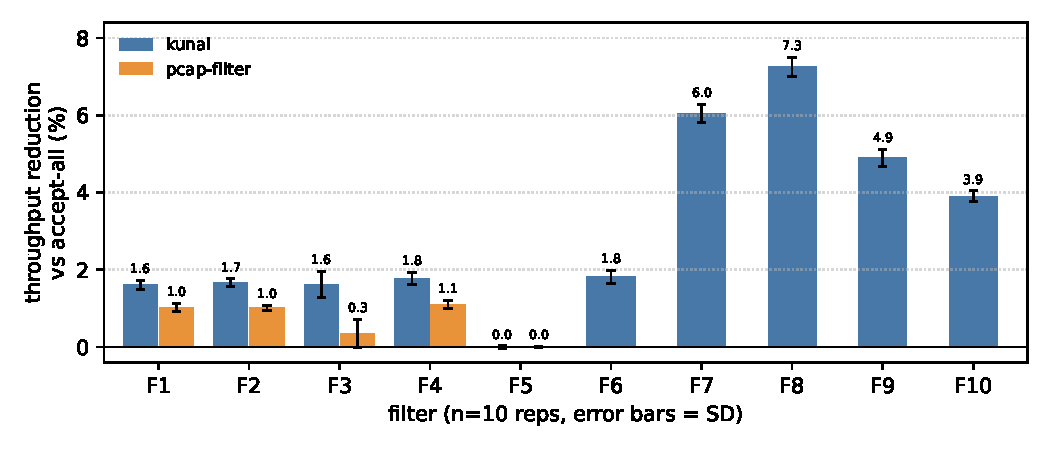
\includegraphics[width=0.62\columnwidth]{figures/fig_datapath.pdf}
  \caption{Datapath processing-rate reduction for F1--F10 (accept-all
  baseline, box plot, $n{=}10$). The heaviest filters (F7 chain walk
  6.6\%, F8 SRv6 loop 7.4\%) are comparable to the 6.7\% window-copy
  cost (dashed); triangles are means.}
  \label{fig:datapath}
\end{figure}

A per-packet run-time measurement via \texttt{BPF\_PROG\_TEST\_RUN}
agreed: over a filterless accept-all baseline of 611--612\,ns, each
filter added at most +15\,ns/pkt (under 3\%), and the
\kunai--pcap-filter difference was at most the measurement standard
deviation. Save for the SRv6 segment loop (F8), whose line-rate cost is
on par with the copy, the cost is dominated by the fixed per-packet work
every program on the datapath shares rather than by filter evaluation.

\section{Limitations}
\label{sec:limitations}

\kunai is a DSL specialized for packet filtering, not a
general-purpose eBPF language: stateful filtering, deep packet
inspection, and aggregation are out of scope, and P4 defines only
header layout and parser transitions, not pipeline mechanisms such as
actions and tables.

\kunai addresses every field by name and offers no escape hatch for a raw
byte offset, as pcap-filter's \texttt{ip[14:2]} does. This
exclusion is deliberate: only a named, schema-resolved access lets the
generator bound each read into a form the verifier accepts, which an
arbitrary run-time offset does not. The raw byte-offset hatch is thus a
one-directional gap by design, not a shortfall.
Sub-byte fields such as a SYN-flag test are still written by name as
\texttt{where tcp.flags \& 0x02 != 0}, with the generator masking a
byte-aligned covering window.

Our verifier-acceptance result is empirical, not a formal guarantee:
we confirmed acceptance and matching on six kernels for F1--F10 and the
regression suite, but acceptance for an arbitrary \kunai expression on
an arbitrary kernel version is future work. Because a variable-length
walk is translated into bounded bytecode, the element count it can walk
has a compile-time bound, and a filter that uses \texttt{bpf\_loop} is
subject to a kernel-version lower bound.

The generated bytecode is only as correct as the protocol definition:
the p4c parse check verifies P4 syntax, not that field offsets or
parser transitions match the relevant RFC. The definitions also have
coverage limits: Geneve option TLVs, for example, are not yet exposed
as filter targets. Finally, \kunai's bytecode is a host-agnostic
evaluator over a packet window, and each host adapter supplies the
layout it sees; at tc, where the kernel moves the outer VLAN tag into
skb metadata, reading that tag value is future work
(\S\ref{sec:eval-accept}).

\section{Conclusion}
\label{sec:conclusion}

We presented \kunai, a verifier-safe packet-filter DSL for nested
encapsulation, repeated protocols, and variable-length structures,
whose bytecode the verifier accepts across six kernels and both attach
points with modest overhead.

\bibliographystyle{ACM-Reference-Format}
\bibliography{refs}

\end{document}
